\documentclass[a4paper, 11pt, twoside]{article}  
\usepackage[hcentering,bindingoffset=10mm,margin=20mm]{geometry}
\usepackage{graphicx}
\graphicspath{{figures/}}  % Location of the graphics files
\usepackage{makeidx}
% \graphicspath{/figures}  % Location of the graphics files
\usepackage{multirow}
% Making R code work!
\usepackage{listings}
\usepackage{color}
\usepackage{hyperref}
\usepackage{booktabs}
\usepackage{float} % allows forcing of float position
% \restylefloat{table}
\usepackage{bm}

% Add toc to contents
\usepackage[nottoc,numbib]{tocbibind}

\hypersetup{urlcolor=blue, colorlinks=false, hypertexnames=true}  % Colours hyperlinks in blue, but this can be distracting 
\usepackage{cleveref}
\definecolor{dkgreen}{rgb}{0,0.6,0}
\definecolor{gray}{rgb}{0.5,0.5,0.5}
\definecolor{mauve}{rgb}{0.58,0,0.82}

\lstset{ %
  language=R,                % the language of the code
   basicstyle=\normalsize\ttfamily,           % the size of the fonts that are used for the code
%   numbers=left,                   % where to put the line-numbers
%   numberstyle=\tiny\color{gray},  % the style that is used for the line-numbers
%   stepnumber=2,                   % the step between two line-numbers. If it's 1, each line
                                  % will be numbered
%   numbersep=5pt,                  % how far the line-numbers are from the code
%   backgroundcolor=\color{white},      % choose the background color. You must add \usepackage{color}
%   showspaces=false,               % show spaces adding particular underscores
%   showstringspaces=false,         % underline spaces within strings
%   showtabs=false,                 % show tabs within strings adding particular underscores
   frame=false,                   % adds a frame around the code
   rulecolor=\color{white},        % if not set, the frame-color may be changed on line-breaks within not-black text (e.g. commens (green here))
%   tabsize=2,                      % sets default tabsize to 2 spaces
%   captionpos=b,                   % sets the caption-position to bottom
%   breaklines=true,                % sets automatic line breaking
%   breakatwhitespace=false,        % sets if automatic breaks should only happen at whitespace
%   title=\lstname,                   % show the filename of files included with \lstinputlisting;
                                  % also try caption instead of title
  keywordstyle=\color{blue},          % keyword style
  commentstyle=\color{dkgreen},       % comment style
  stringstyle=\color{mauve},         % string literal style
  escapeinside={\%*}{*)},            % if you want to add a comment within your code
  morekeywords={*,...}               % if you want to add more keywords to the set
} 

% Include any extra LaTeX packages required
\usepackage[round,]{natbib}  % Use the "Natbib" style for the references
\usepackage{verbatim}  % Needed for the "comment" environment to make LaTeX comments
\usepackage{wallpaper}
\usepackage{cases}
\usepackage{wrapfig}
\makeindex
% \renewcommand{\includegraphics}[2][]{\fbox{#2}} %omits images
\begin{document}
 
\title{Introducing spatial microsimulation with R: a practical}
% \author{Robin Lovelace --- R.Lovelace at. Leeds. ac. uk}
\pagestyle{myheadings}
\author{Lovelace, Robin\\
\texttt{r.lovelace@leeds.ac.uk}}
\maketitle

\tableofcontents

\newpage
\section{Foundations}

\subsection{Prerequisites for this practical}

This practical is about spatial microsimulation in the software
R. We suggest you install and take a look at this powerful program
before getting started. We recommend using R within RStudio, which makes
using R much easier. Instructions to install both R and RStudio can be found
online: \href{http://www.rstudio.com/ide/download/desktop}{rstudio.com/ide/download/desktop}.

The other prerequisite for the course is downloading the example data.
These can be downloaded in a single zip file which can be found on the
course's GitHub repository: \\*
\href{https://github.com/Robinlovelace/smsim-course}{github.com/Robinlovelace/smsim-course}.
Click on the ``Download ZIP'' button to the right of this page and extract
the folder into your desktop or other suitable place on your computer.
% Could add screenshot of Dl ZIP here!!!

\begin{wrapfigure}{2}{9cm}
\begin{center}
   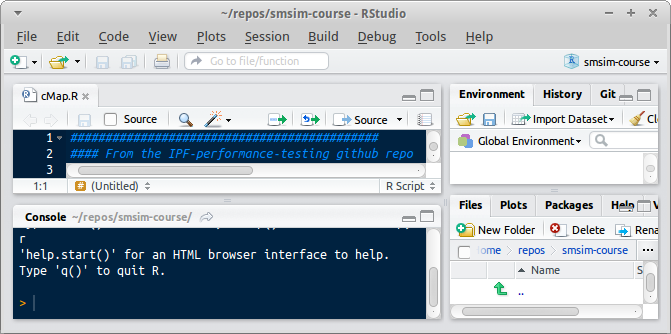
\includegraphics[width=9cm]{rstudio}
\end{center}
 \caption{The RStudio user interface. Note the project title `smsim-course' in
the top right and the `Files' tab at the top of the left hand window.}
\label{frstudio}
\end{wrapfigure}

Once the folder has been successfully extracted open it in
your browser and take a look around. You will find a number of files
and two sub-folders
entitled `data', and `figures'. When you get to the
sections that use R code, it is useful for R to operate from
within the smsim-course-master folder. Probably the best way
to set this up is to open the file `smsim-course.Rproj' from
within RStudio (\cref{frstudio}).
Try this now and click on the `Files' tab in
the bottom right hand window of RStudio.
Before using the power of R in RStudio it's worth
understanding a bit about `IPF', the algorithm we will use to generate
the synthetic population or `spatial microdata' (\cref{fmsim-schema}).

\subsection{Learning by doing}

As \citet[xxii]{kabacoff2011r} put it regarding R, ``the best
way to learn is to experiment'' and the same applies to spatial microsimulation.
We believe you will learn the technique/art best not by reading about it, 
but by doing it. Mistakes are inevitable in any challenging task and should not
be discouraged. In fact it is by making blunders, identifying and then correcting them
that many people learn best. Think of someone learning to skate: no one ever
picks up a skateboard for the first time being able to `surf the sidewalks'. It
takes time, patience and plenty of falls before you master the art.
The same applies to spatial microsimulation.

One of the tricky things about spatial microsimulation for newcomers is its use
of specialist language. It is important to know exactly what is meant by
`special microdata' and other technical terms. To this end we have created a
glossary that provide succinct definitions (see \cref{gloss}). Any term that is
\emph{italicised} in the text has a glossary entry.

Spatial microsimulation works by taking \emph{microdata} at the individual level
and using aggregate-level constraints to allocate these individuals to zones.
The two main methods are \emph{deterministic reweighting} and \emph{combinatorial optimisation}.
This practical takes the former approach using a process called \emph{iterative proportional fitting}
(IPF). IPF is used to increase the weights of individuals who are representative
of the target area and reduce the weights of individuals who are relatively
rare \citep{Lovelace2013-trs}.
The output is a \emph{spatial microdataset}.

A schematic of the process is shown in \cref{fmsim-schema}.
Take a look at the image and think about the process. But we don't want to get
bogged down in theory or applications in this course: we want to `get our
hands dirty'. Next we will do just that, by applying the process to some
example data.

\begin{figure}[H]
\begin{center}
  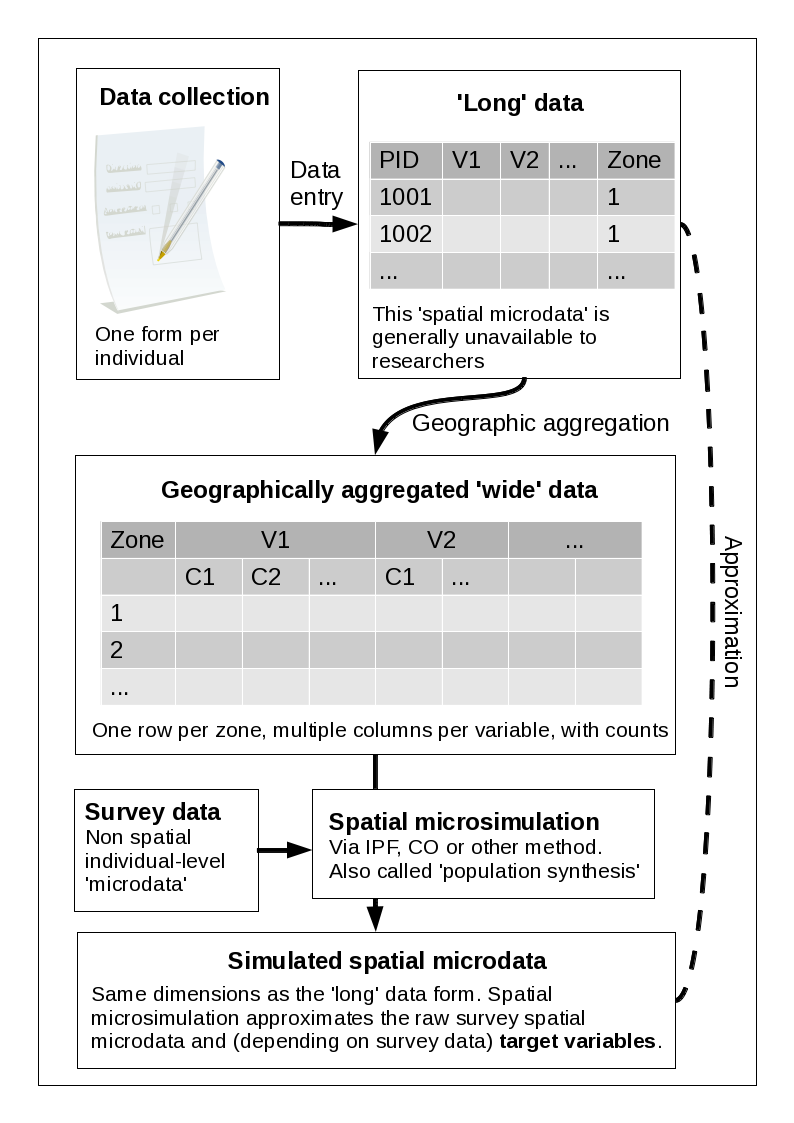
\includegraphics[width=9cm]{msim-schema}
\end{center}
\caption{Schema of iterative proportional fitting (IPF) and combinatorial
optimisation
in the wider context of the availability of different data formats and spatial
microsimulation. \label{fmsim-schema}}
\end{figure}


\subsection{Some input data} \label{s:theory}

Let's start with a very basic dataset. To aid understanding, we will first do
the reweighting by hand
to understand the process before automating it on the computer.
Table \ref{t:w} shows 5 individuals, who are defined by two
constraint variables: age and sex.
Table \ref{t:s} contains data for a hypothetical area. \Cref{t:s2} illustrates
this aggregate level table in a different form,
to show our ignorance of interaction between age and sex. Finally, table
\ref{t:m} presents the hypothetical microdata in aggregated form,
that can be compared directly to the aggregate data presented in
Table \ref{t:s2}.

\begin{table}[h]
% {r}{10cm}
\caption{A hypothetical input microdata set
% (the original
% weights set to one). The bold value is used subsequently for
% illustrative purposes.
}
\label{t:w}
\begin{center}
 \begin{tabular}{llll}
\toprule
{Individual } & {Age} & {Sex}  & {Weight} \\
\midrule
1 & 59 & Male  & 1 \\
2 & 54 & Male & 1 \\
3 & {35} & {Male} & \textbf{1} \\
4 & 73 & Female & 1 \\
5 & 49 & Female & 1 \\
% 1 & 59 & m \\
% 2 & 54 & m \\
% 3 & 35 & m \\
% 4 & 73 & f \\
% 5 & 49 & f \\
\bottomrule
\end{tabular}
\end{center}
\end{table}

\begin{table}[H]
\centering{
\caption{Small area constraints ($s$). \label{t:s}}
\begin{tabular}{cllll}
\toprule
Constraint $\Rightarrow$ & \multicolumn{2}{c}{$i$}& \multicolumn{2}{c}{$j$}\\
Category $\Rightarrow$ & $i_1$ & $i_2$ & $j_1$ & $j_2$ \\
Area $\Downarrow$  & Under-50 & Over-50 &  Male & Female\\
1  & \textbf{8} & 4 & 6 & 6\\
\bottomrule
\end{tabular}}
\end{table}
\vspace{1cm}

\begin{table}[h]
\centering
\caption[Small area constraints expressed as marginal totals]{Small
area constraints expressed as marginal totals, and the cell
values to be estimated.}
\begin{tabular}{cllll}\toprule
Marginal totals&  & \multicolumn{2}{c}{$j$} & \\
& Age/sex & Male & Female & T\\ \midrule
\multirow{2}{*}{$i$} & Under-50 & \textbf{?} & ? & \textbf{8}\\
& Over-50 & ? & ? &4 \\
& T & 6 & 6 &12\\
\bottomrule
\end{tabular}
\label{t:s2}
\end{table}

\begin{table}[htbp]
\centering
\caption[The aggregated results of the weighted
microdata set]{The aggregated results of the weighted
microdata set ($m(1)$).
Note, these values depend on the
weights allocated in Table \ref{t:w} and therefore
 change after each iteration}

\begin{tabular}{cllll}\toprule
Marginal totals&  & \multicolumn{2}{c}{$j$} & \\
& Age/sex & Male & Female & T\\ \midrule
\multirow{2}{*}{$i$} & Under-50 & \textbf{1} & 1 & \textbf{2}\\
& Over-50 & 2 & 1 &3 \\
& T & 3 & 2 &5\\
\bottomrule
\end{tabular}
\label{t:m}
\end{table}

\subsection{The IPF equation} \label{ipfeq}

\begin{wrapfigure}{R}{9cm}
   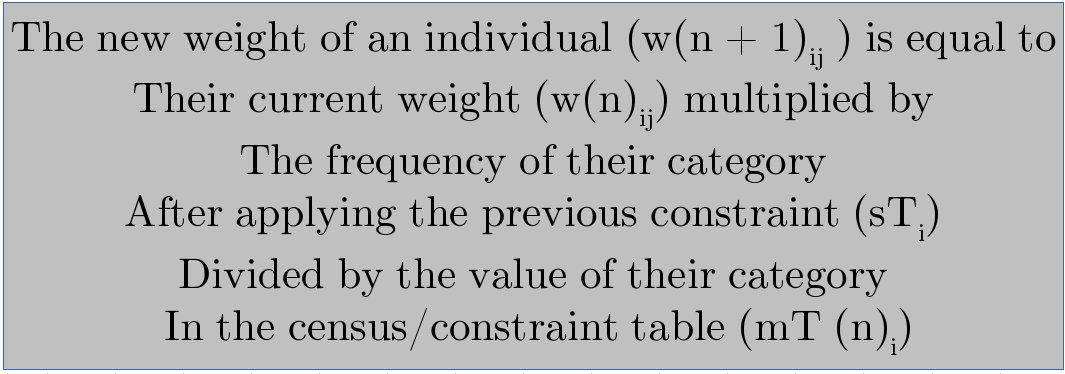
\includegraphics[width=8cm]{equation1}
 \caption{\Cref{eq:ipf} in word form.}
\label{feq}
\end{wrapfigure}

Using these tables we readjust the weights of the
individuals so that their sum equals the total population of the area presented
in Table \ref{t:s2}.
For each constraint, the weights are multiplied
by the aggregate level values from Table \ref{t:s} and divided by the
respective marginal total of the microdata (see \cref{t:m}).
This is done one constraint at a time, as described in
\cref{feq} and more formally by
\cref{eq:ipf} for constraint $i$ (age in this case):



\begin{equation}
w(n+1)_{ij} = \frac{w(n)_{ij} \times sT_{i}}{mT(n)_{i}}
\label{eq:ipf}
\end{equation}



where $w(n+1)_{ij}$ is the new weight for individuals with characteristics $i$
(age, in this case), and $j$ (sex),  $w(n)_{ij}$ is the original
weight for individuals with these characteristics, $sT_{i}$ is element
marginal total of the small area constraint, $s$
(Table \ref{t:s}) and $mT(n)_{i}$ is the marginal total of category
$j$ of the aggregated results of the weighted
microdata, $m$ (Table \ref{t:m}).
$n$ represents the iteration number.


Do not worry about understanding the above equation for now.
More important is implementing it. Follow the emboldened values in tables 1 to 4
to see how the new weight of individual 3 is calculated for the age constraint.
Table \ref{t:new-weights} illustrates the outcome. Notice that the
sum of the weights is equal to the total population, from the constraint variables.

\begin{table}[htbp]
\centering
\caption{Reweighting the hypothetical microdataset in order to fit
Table \ref{t:s}.}
\begin{tabular}{lllll}
\toprule
{Individual} & {Sex} & {age-group} & {Weight} &
{New weight, w(2)} \\ \midrule
1 & Male & Over-50 & 1 & $1 \times 4/3 = \frac{4}{3}$ \\
2 & Male & Over-50 & 1 & $1 \times 4/3 = \frac{4}{3}$ \\
3 & Male & Under-50 & 1 & $\textbf{1} \times
\textbf{8}/\textbf{2} = 4$ \\
4 & Female & Over-50 & 1 & $1 \times 4/3 = \frac{4}{3}$ \\
5 & Female & Under-50 & 1 & $1 \times 8/2 = 4$ \\
\midrule
Total & & & 5 & 12 \\
\bottomrule
\end{tabular}
\label{t:new-weights}
\end{table}

After the individual level data have been re-aggregated (\cref{t:m2}),
the next stage is to repeat \cref{eq:ipf} for the age constraint to generate a
third set of weights, by replacing
the $i$ in $sT_{i}$ and $mT(n)_{i}$ with $j$ and incrementing the value of n:

\begin{equation}
w(3)_{ij} = \frac{w(2)_{ij} \times sT_{j}}{mT(2)_{j}}
\label{eq:ipf2}
\end{equation}

\subsection{Test your understanding}
To test your understanding of IPF, try to apply \cref{eq:ipf2} to the
information above
and that presented in \cref{t:m2}.
This should result in the following vector of new weights, for individuals 1 to
5. Calculate the correct values and pencil them in in place of the question
marks.  % Add online link to answers - tinyurl


\begin{equation}
w(3) = (\frac{6 \times \frac{4}{3}}{6 \frac{2}{3}}, \frac{6 \times
\frac{4}{3}}{?}, \boldsymbol{ \frac{4 \times 6}{ 6\frac{2}{3}
}}, \frac{?}{?}, \frac{4 \times 6}{5 \frac{1}{3}})
% w(3) = (\frac{6}{5}, \frac{6}{5}, \frac{18}{5}, \frac{3}{2}, \frac{9}{2})
\end{equation}

After simplifying these fractions, the results are as follows.
One `sanity' check of your method here is whether the sum of these
weights is still equal to the area's total population of twelve. Test this is
true:

\begin{equation}
% w(3) = (\frac{6}{5}, \frac{6}{?}, \boldsymbol{ \frac{4 \times 6}{ 6\frac{2}{3}
% }}, \frac{?}{?}, \frac{9}{2})
w(3) = (\frac{6}{5}, \frac{6}{5}, \boldsymbol{\frac{18}{5}}, \frac{3}{2},
\frac{9}{2})
\label{finalout}
\end{equation}

What do the weights in w(3) actually mean? They indicate how representative
each individual is of the target zone after one iteration of IPF, constraining
by age and sex. Individual number 5 has the highest weight because there is
only one young female in the survey dataset yet seemingly many in the area in
question.

Notice also that after each iteration the fit between the marginal
totals of $m$ and $s$
improves.\footnote{This can be checked by comparing the aggregated weighted
individuals with the small area constraints. Total absolute error (TAE),
defined as the sum of all differences between simulated and observed marginal
totals, improves between $m(1)$ to $m(2)$, falling from
14 to 6 in \cref{t:m} and \cref{t:m2} above. TAE for $m(3)$ (not shown,
but calculated by aggregating $w(3)$) improves even more, to 1.3.
This number would eventually converge to 0 through subsequent
iterations, a defining feature of IPF.}


\begin{table}[htbp]
\centering
\caption[Aggregated results after constraining for age]{The
aggregated results of the weighted
microdata set after constraining for age ($m(2)$).
}

\begin{tabular}{cllll}\toprule
Marginal totals&  & \multicolumn{2}{c}{$i$} & \\
& Age/sex & Male & Female & T\\ \midrule
\multirow{2}{*}{$j$} & Under-50 & \textbf{4} & 4 & 8\\
& Over-50 & $\frac{8}{3}$ & $\frac{4}{3}$ & 4 \\
& T & $\boldsymbol{6\frac{2}{3}}$ & 5$\frac{1}{3}$ & 12\\
\bottomrule
\end{tabular}
\label{t:m2}
\end{table}

% A key benefit from a policy perspective is that
% IPF and other spatial microsimultion techniques
% can provide estimation of variables whose values are not
% known at the local level (e.g. income).

\subsection{IPF in a spreadsheet}
% Computer code is absent from most people's daily lives so the
% R code we use to automate IPF will likely seem like a foreign language
% to many. Spreadsheet programs like Microsoft Excel and LibrOffice Calc are
% comparatively well known, though.
To ensure smooth transition between the IPF process
described in mathematics above and its implementation in R this section
provides an intermediary stage: the speed of computation and the visual support
of a graphical user interface (GUI).


\subsection{IPF in R: a simple example} \label{simplementing}
% priority: automate!!!
So far we have implemented IPF by hand and in a spreadsheet.
This section explains how the IPF
\emph{algorithm} described above is implemented in R, using the
same input data.\footnote{A fuller tutorial is available from Rpubs, a site dedicated
to publishing R analyses that are reproducible. This tutorial uses the RMarkdown
mark-up language, which enables R code to be run and presented within
documents. See http://rpubs.com/RobinLovelace/5089 \label{fnrpub} .}
% This section is based on ``Spatial microsimulation in R: a
% beginner’s guide to iterative proportional fitting (IPF)'', a tutorial
% written to accompany a methods paper on integerisation
The code snippets are taken from the `simple.R' script file (just a plain text
document, like all R scripts) so you can copy and paste. However, it is
highly recommended to not look at this file until you need to, towards
the end of
section. This is `leaning by typing'!

The data presented in the above worked example are saved in the
`simple' sub-folder of `data' as .csv files. To load them in R,
we use the following commands:

\begin{lstlisting}[float=h, caption={Loading the input data in R}, label=cusd]
ind <- read.csv("data/simple/ind.csv") # load the individual level data
cons <- read.csv("data/simple/cons.csv") # load aggregate constraints
\end{lstlisting}

To check that the \emph{data frames} have loaded correctly, simply
ask R to print their contents by entering the object's name. To display the
individual level data, for example, simply type the
following:\footnote{An alternative
way to do this is to click on the object's name in the `Environment' tab in
RStudio's top right window.}

\begin{lstlisting}[float=h, caption={Checking the contents of the individual
level data frame}, label=cout]
ind # Show the data frame in R
##  id age sex
##   1  59   m
##   2  54   m
##   3  35   m
##   4  73   f
##   5  49   f
\end{lstlisting}

Note that the input data is identical to the tables illustrated above for
consistency. Instead of constraining for just one zone as we did in the example
above, we will fit the data to six zones here. To subset a dataset, add square
brackets to the end of the object's name in R. Entering \verb cons[1:2,] ,
for example, should output the first two rows of the constraint variable.
Within the square brackets the number before the comma refers to columns (blank
means all columns) and the numbers after the comma refer to rows. If the output
of this command looks like the text below, congratulations are in order:
you have successfully loaded the constraint dataset.

\begin{lstlisting}[float=h, caption={Printing a subset of the constraint data
in R},
label=cou]
cons[1:2,]
##    X16.49 X50. m f
##  1      8    4 6 6
##  2      2    8 4 6
\end{lstlisting}

Note that the top row is identical to \cref{t:s} --- we can therefore compare
the results of doing IPF on the computer with the results obtained by hand.

% !!! Manual input of data for book!!!
% Usually the input data for spatial microsimulation are loaded from
%  .csv files, one for each
% constraint and one for the input microdata. These are read-in with the command
% \verb read.csv . For the purposes of understanding how the model works,
% the dataset is read line by line, following the
% example above. The following code creates example datasets,
% based on the same hypothetical survey of 5 individuals described above,
% and 5 small areas. The spatial microsimulation model will select individuals
% based on age and sex and mode of transport (mode of transport
% is also used on the larger online example described in footnote \ref{fnrpub}).
% For consistency with the (larger) model used for the paper, 
% the individual level data will be referred to as USd (Understanding Society dataset)
% and the geographic data as all.msim (for all constraint variables).
% The code to read-in the individual level data are presented in code sample \ref{cusd}.
% When called, the data are then displayed as a table (see listing \ref{cout}).
% \begin{lstlisting}[float=h, caption={Manual input of individual level data
% in R}, label=cusd]
% # Read in the data in long form (normaly read.table() used)
% c.names <- c("id", "age", "sex")
% USd <- c(       1, 59, "m",
%                 2, 54, "m",
%                 3, 35, "m",
%                 4, 73, "f",
%                 5, 49, "f")
% USd <- matrix(USd, nrow = 5, byrow = T) # Long data into matrix
% USd <- data.frame(USd) # Convert this into a dataframe
% names(USd) <- c.names # Add correct column names
% USd$age <- as.numeric(levels(USd$age)[USd$age]) # Age is a numeric
% \end{lstlisting}
% \begin{lstlisting}[float=h, caption={Output of the USd data frame}, label=cout]
% USd # Show the data frame in R
% ##   id age sex
% ## 1  1  59   m
% ## 2  2  54   m
% ## 3  3  35   m
% ## 4  4  73   f
% ## 5  5  49   f
% \end{lstlisting}
% The same procedure applies to the geographical data (listing \ref{cgeo}).
% \begin{lstlisting}[float=h*, caption={Geographic data input}, label=cgeo]
%  category.labels <- c("16-49", "50+" # Age constraint
%              ,"m", "f" # Sex constraint
%              # more constraints could go here
%              )
% all.msim <- c(  8, 4,    6, 6,   # Original aggregate data
%                 2, 8,    4, 6,   # Elderly
%                 7, 4,    3, 8,   # Female dominated
%                 5, 4,    7, 2,   # Male dominated
%                 7, 3,    6, 4    # Young
%                 )
% all.msim <- matrix(all.msim, nrow = 5, byrow = T) 
% all.msim <- data.frame(all.msim) # Convert to dataframe
% names(all.msim) <- category.labels # Add correct column names
% \end{lstlisting}

% IPF relies on the assumption that all constraint variables will contain the
% same number of people. This is logical (how can there be more people classified
% by age than by sex?) but can cause problems for constraint variables that use
% only a subset of the total population, such as those who responded to questions on
% travel to work. To overcome this problem, it is possible to normalise the
% constraint variables, setting the total for each to the one that has the most
% reliable total population. This worked example simply checks whether
% or not they are (listing \ref{ccheck}).

% \begin{lstlisting}[float=h, caption={R code to check the constrain populations
% match}, label=ccheck]
%  # Check totals for each constraint match
% rowSums(all.msim[,1:2]) # Age constraint
% ## [1] 12 10 11  9 10
% rowSums(all.msim[,3:4]) # Sex constraint
% ## [1] 12 10 11  9 10
% 
% rowSums(all.msim[,1:2]) == rowSums(all.msim[,3:4])
% ## [1] TRUE TRUE TRUE TRUE TRUE
% \end{lstlisting}

To make the individual level data comparable to the aggregate level we must
first categorise it and count the number in each category. This job is
performed by the R \emph{script} categorise.R, contained in the `simple' data
folder. Run it by entering
\verb source("data/simple/categorise.R")) . This results in the creation of a
new object called ind.cat, which converts the variables into a matrix of 0s and
1s with same number of columns as the constraint data. Note that the
`categories.R' script must be modified each time it is used with a different
dataset. To check that the script has worked
properly, lets count the number of individuals it contains:

\begin{lstlisting}[float=h, caption={Output from ind.cat}]
colSums(ind.cat)
##    a16.49   a50.      m      f
##         2      3      3      2 
\end{lstlisting}

The sum of both age and sex variables is 5 (the total number of individuals): it
worked! Now the data is in the same form as the constraint variables and we
have checked the data makes sense, we can create the `weight' matrix and begin
reweighting the individuals to
zones:\footnote{The
above code will probably seem
daunting and not make sense unless
you are an experienced R user. Do not worry about this for now, you can always
check what is going on later by checking R's documentation (e.g. try entering
`?rep') or
by pressing the tab key when entering arguments for R commands. For the time
being, it is best to press-on with the example and understand the concepts ---
the details can be looked at later.}

\begin{lstlisting}[float=h, caption={Creating the weight and aggregated
individual level matrices}]
weights <- array(1, dim=c(nrow(ind),nrow(cons)))
ind.agg <- matrix(rep(colSums(ind.cat), nrow(cons)), nrow(cons))
\end{lstlisting}

With all of these objects in place, we are ready to begin allocating new weights
to the individuals via IPF. Below is written in code the IPF formula presented
in \cref{ipfeq}.

\begin{lstlisting}[float=h, caption={Creating new weights for the individuals
based on constraint 1 (age) via IPF}]
for (j in 1:nrow(cons)){
  for(i in 1:ncol(con1)){
 weights[which(ind.cat[,i] == 1),j] <- con1[j,i] / ind.agg[j,i]}}
\end{lstlisting}

The above code creates the weight matrix that allocates individuals to zones.
Aggregating this data to zones allows us to update `ind.agg' with new values
that will be closer to the constraint variables. This is verified in the `simple.R'
script file with a line of code that calculates the Total Absolute Error
after each iteration --- \verb sum(sqrt((ind.agg-cons)^2)) .
Check the error decreases with each iteration.

At this stage you should switch to running the code in `simple.R'. In RStudio
to run a line of code from the top left window, simply press \verb Ctl-Enter .
Use this technique to constrain by the second constraint, sex.
Notice that we have just done in code what was previously done by
hand. % TODO: and in a spreadsheet!
Thus we can verify the output of the R implementation against 
that obtained through mental arithmetic. Compare
the following listing with \cref{finalout}: are the weights the same?

\begin{lstlisting}[float=h, caption={W(3) after constraining by age and sex in R. 
Compare with \cref{finalout}}]
weights3[,1] # check the weights allocated for zone 1
##    [1] 1.2 1.2 3.6 1.5 4.5
\end{lstlisting}

\newpage
\subsection{Iterations}

In the above example, we have seen the `bare bones' of spatial microsimulation
using IPF to generate weights from which sample populations can be created.
To perform multiple iterations of the same model, we have prepared a slightly
more complex script than `simple.R' called `etsim.R' that can be found in the
`data/simple/' folder. Th etsim script
generates weights for as many iterations as you please (just
change the value of \verb num.its ). This happens by calling another
script called `e2.R' which is simply run repeatedly for each iteration. 

There
is great scope for taking the analysis further:
some further tests and plots are presented on the on-line
versions of this section. The simplest case is contained in
Rpubs document \href{http://rpubs.com/RobinLovelace/6193}{rpubs.com/RobinLovelace/6193} 
and a more complex case (with three constraints) can be found in Rpubs document
\href{http://rpubs.com/RobinLovelace/5089}{5089}. For now, however,
we progress to a more complex example, CakeMap.

\section{CakeMap: A worked example}

In this section we will process real data to arrive at an important result:
an estimate of the amount of cake eaten in different wards in West Yorkshire. The
example is deliberately rather absurd: hopefully this will make
the technique more memorable. An attempt has been made to present the method
in a generalisable was as possible, allowing users to apply the technique described
here to their own data.

The code needed to run the main part of the example is contained within `cakeMap.R'.
Note that this script makes frequent reference to files contained in the `cakeMap'
folder `data'. \verb read.csv("data/cakeMap/ind.csv") , for example, is used to read
the individual level data into R.

Because this example uses real world data (albeit in anonymised form),
we will see how important the process of `data cleaning' is.
Rarely are datasets downloaded in exactly the right form for them to
be pumped directly into a spatial microsimulation model. For that reason
we describe the process of loading and preparing the input data first:
similar steps will be needed to use your own data as an input into a
spatial microsimulation model.

\subsection{Loading and preparing the input data}

The raw constraint variables for CakeMap were downloaded from
the Infuse website (\href{http://infuse.mimas.ac.uk/}{infuse.mimas.ac.uk/}).
These, logically enough, are stored in the `cakeMap/data/' directory
as .csv files and contain the word `raw' so it is clear which files
contain the raw data. The file `age-sex-raw.csv', for example is the raw
age and sex data that was downloaded. As the screenshot in \cref{fraw} shows,
it was provided in a rather verbose form and needed to be
processed before it could be usefully used as an input
in a spatial microsimulation model. `con1.csv' stands for
`constraint 1' and represents this age/sex data after it has been processed.

\begin{figure}
 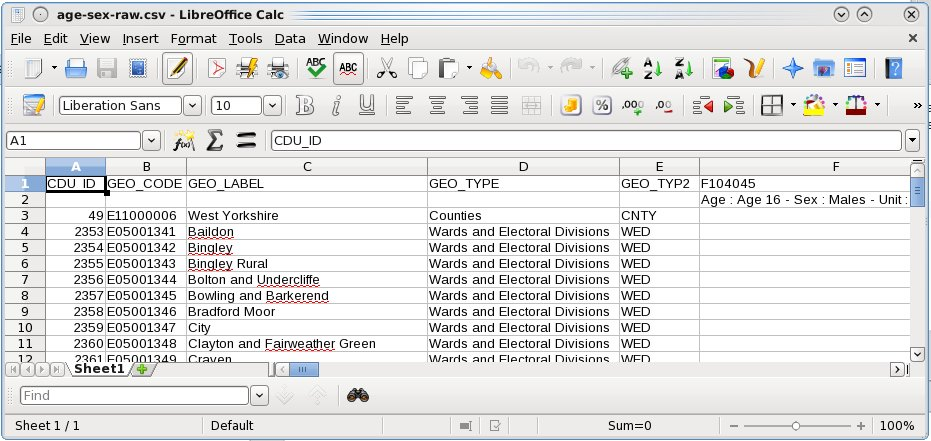
\includegraphics[width=12cm]{raw-data-screenshot}
\caption{The raw input data for the CakeMap model, downloaded from the InFuse website.}
\label{fraw}
\end{figure}


To ensure reproducibility in the process of converting the raw data into
this `spatial microsimulation ready' dataset, all of the steps used to
clean and rearrange the data have been saved. Take a look at the R script file
`process-age.R' --- these are the kinds of steps that the researcher will need to
undertake before performing a spatial microsimulation model. 
Here is not the place to delve into the details of data reformatting;
there are resources dedicated to that \citep{tidy-data, kabacoff2011r}.
However, it is worth taking a look at the `process-age.R' script and the
other `process*' files to gain insight into how R can be used to quickly
and effectively be used to process complex raw data into a form that is
ready for use in modelling work.

The input data generated through this process of data preparation are named
`con1.csv' to `con3.csv'. For simplicity, all these were merged into a single
dataset called `cons.csv'. All the input data for this section
are loaded with the following commands:


\begin{lstlisting}[float=h, caption={Loading the input data for CakeMap (see `cMap.R')}]
ind <- read.csv("data/cakeMap/ind.csv")
cons <- read.csv("data/cakeMap/cons.csv")
\end{lstlisting}

Take a look at these input data using the techniques learned in the previous
section. To test your understanding, try to answer the following questions:
what are the constraint variables? How many individuals are in the survey microdataset?
How many zones will we generate spatial microdata for?

For bonus points that will test your R skills as well as your practical knowledge
of spatial microsimulation, try constructing queries in R that will automatically
answer these questions.

It is vital to understand the input datasets before trying to model them, so
take some time exploring the input. Only when satisfied with your understanding of
the datasets (a pen and paper can help here, as well as R!) is it time
to move on to generate the spatial microdata using IPF.

\subsection{Performing IPF on the CakeMap data}

\subsection{Processing the output}

\subsection{Mapping the results}
\section{Applying the technique in the real world} \label{smeval}
Here we will continue with the cakeMap model we ran in the previous section.

\subsection{Model checking and validation}
To make an analogy with food safety standards, openness about mistakes is
conducive to high standards \citep{Powell2011}. Transparency in model
verification is desirable for similar reasons. The two main strategies are 1) 
comparing the model results with knowledge of how it \emph{should}
perform \emph{a-priori} (model checking) and 2) comparison between the model
results and empirical data (validation).

A proven method of checking that data analysis and processing is working
is wide ranging and continual visual exploration of its output
\citep{janert2010data}.

% \subsection{Model validation}
% \label{meval}
% % {\color{red} Should this section be in a later chapter?} !!!
Beyond typos or simple conceptual errors in model code, more fundamental
questions should be asked of spatial microsimulation models. The validity
of the assumptions on which they are built, and the confidence one should have
in the results are important.

\subsection{Visualising the results}
Visualisation is an important part of communicating quantitative
data, especially so when the datasets are large and complex so not
conducive to description with tables or words.

Because we have generated spatial data, it is useful to create 
a map of the results, to see how it varies from place to place.
The code used to do this found in `cMapPlot.R'. A vital function within
this script is `merge', which is used to add the simulated cake data
to the geographic 
dataframe:\footnote{`join'
is an alternative to merge from the `plyr' package also used
in the `cMapPlot.R' script that performs the
same task. Assuming `plyr' is loaded --- `library(plyr)' you can read
more about join by entering `?join' in R.}

\begin{lstlisting}[float=h, caption={The merge function for joining
the spatial microsimulation results with geographic data. 
Compare with \cref{finalout}}]
merge(wardsF, wards@data, by = "id")
\end{lstlisting}

The above line of code by default selects all the data
contained in the first object (`wardsF') and adds to it new variables
from the second object based on the linking variable (in this case ``id'').
Also in that script file you will encounter the function \verb fortify ,
the purpose of which is to convert the spatial data object into a
data frame. More on this process is described in \citet{lovelace2014introduction}.
The final map result of `cakeMapPlot.R' is illustrated below (\cref{fcmap}).

\begin{figure}
 \centering
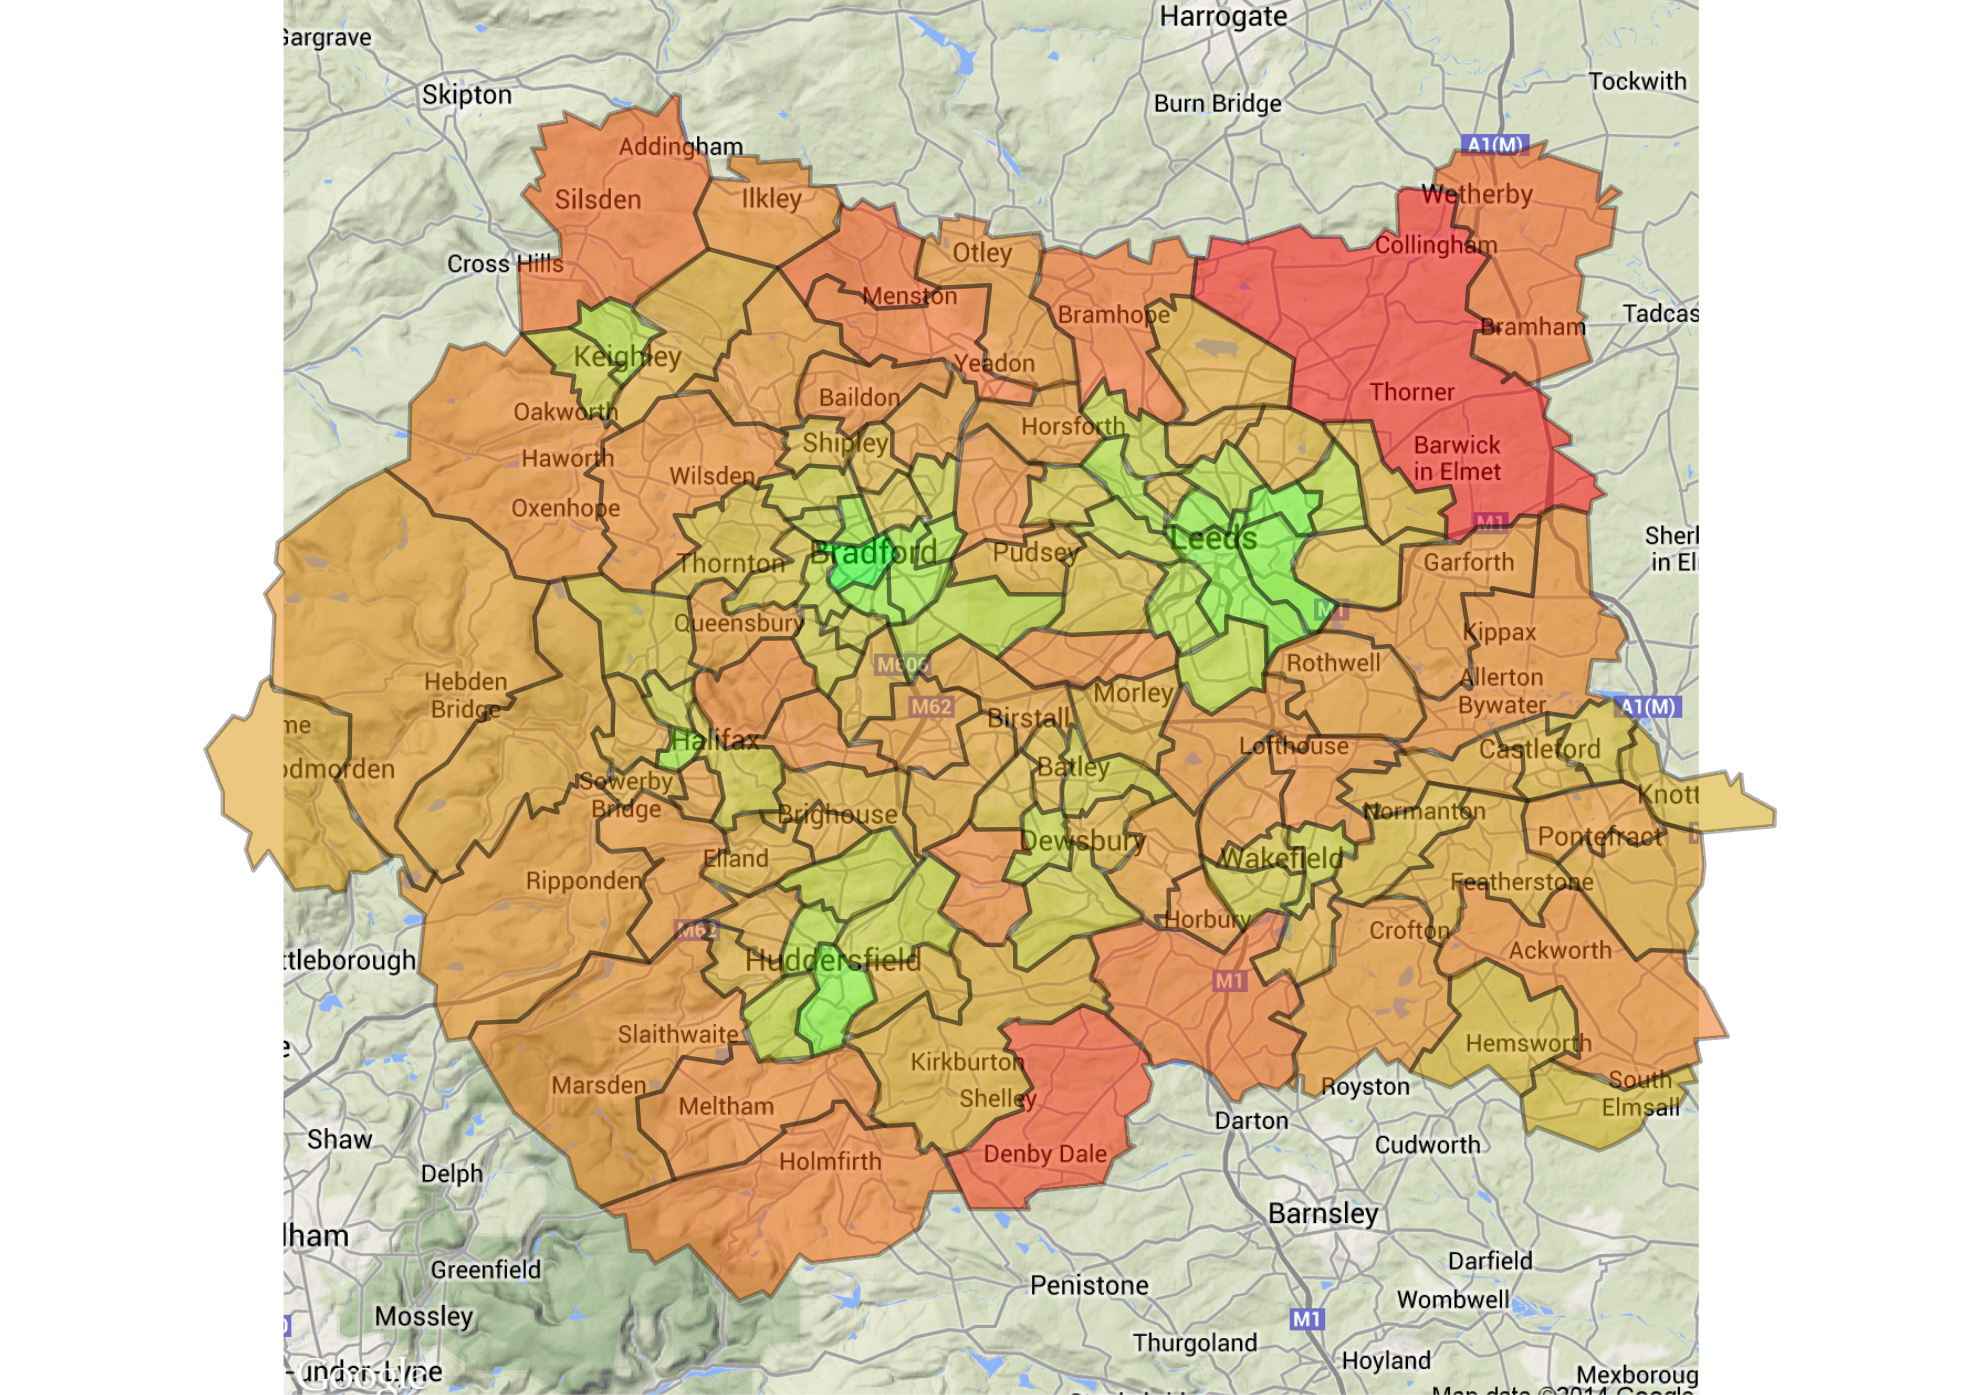
\includegraphics[width=12cm]{cakeMap}
\caption{Choropleth map of the spatial distribution of average frequency of
cake consumption in West Yorkshire, based on simulated data.} 
\label{fcmap}
\end{figure}

\subsection{Analysis}

Once a spatial microdataset has been generated that we are happy with,
we will probably want to analyse it further. This means exploring it --- its main features,
variability and links with other datasets. To illustrate this process we will
load an additional dataset and compare it with the
estimates of cake consumption per person  generated in the previous
section at the ward level.  

The hypothesis we would like to test is that cake consumption is linked to deprivation:
More deprived people will eat unheathily and cake is a relatively cheap `comfort food'.
Assuming our simulated data is correct ---  a questionable assumption but lets roll with
it for now --- we can explore this at the ward level thanks to a 
\href{http://www.neighbourhood.statistics.gov.uk/dissemination/instanceSelection.do?JSAllowed=true&Function=&%24ph=61&CurrentPageId=61&step=2&datasetFamilyId=266&instanceSelection=121427&Next.x=22&Next.y=13&nsjs=true&nsck=false&nssvg=false&nswid=1920}{dataset on 
modelled income from neighbourhood statistics}.

Because the income dataset was produced for old ward boundaries (they were slightly
modified for the 2011 census), we cannot merge with the spatial dataset based on the
new zone codes. Instead we rely on the name of the wards. The code below provides a
snapshot of these names and demonstrates how they can be joined using the `join' function.

\begin{lstlisting}[float=h, caption={The merge function for joining
the spatial microsimulation results with geographic data. 
Compare with \cref{finalout}}]
wards@data <- join(wards@data, imd)
summary(imd$NAME %in% wards$NAME)
##       Mode   FALSE    TRUE    NA's 
##    logical      55      71       0 
\end{lstlisting}

The above code first joins the two datasets together and then checks the result by
seeing how many matches names there are. In practice the fit between old names and new
names is quite poor: only 71 out of 124. In a proper analysis we would have to solve this
problem (e.g. via the command \verb pmatch ~ whhich stands for partial match).
For the purposes of this excercise we will simply plot income against
simulated cake consumption to gain a feeling what
it tells us about the relationship between cake consumption and wealth (\cref{incomeCake}).

\begin{figure}
\centering
 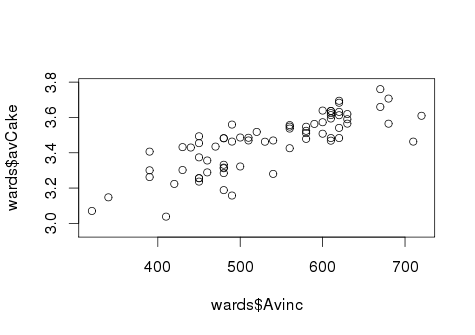
\includegraphics[width=7cm]{incomeCake}
\caption{Relationship between modelled average ward income and
 simulated number of cakes eaten per person per week.}
\label{incomeCake}
\end{figure}

The question raised by this finding is: why? 
Not why is cake consumption higher in wealthy areas (this has not
been established) but: why has the model resulted in this correlation?
To explore this question we need to go back and look at the individual
level data. The most relevant constraint variable for income was class.
When we look at the relationship between social class and cake consumption
in the Dental Health Survey, we find that there is indeed a link:
individuals in the highest three classes (1.1, 1.2, 2) have an average
cake intake of 3.9 cakes per week whereas the three lowest classes have
an average intake of 3.7. This is a relatively modest difference but,
when averaging over large areas, it helps explain the result.
The class dependence of cake consumption in the Dental Health Survey is
illustrated in \cref{hm}.

\begin{figure}
\centering
 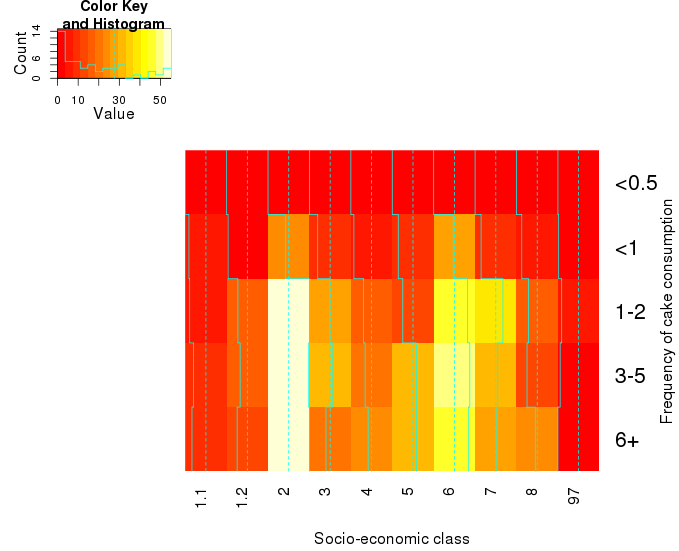
\includegraphics[width=11cm]{hm}
\caption{Relationship between social class and cake consumption in the
individual level data.}
\label{hm}
\end{figure}

\section{Discussion}

What have we learned during the course of this practical tutorial?
Given that it was geared towards beginners, from one perspective
one could say `not a lot' relative to the many potential applications.
The emphasis on understanding of the basics was deliberate: it is only
on strong foundations that large and long-lived buildings can be 
constructed and the same applies to geographical research.

The focus on strong foundations is also sensible because the
number of people actively involved in spatial microsimulation research,
let alone development of new software and methods, is very small.
Specialist skills and understanding is needed to join this research area
and a central outcome of this course has been to provide these.
More specifically, we have learned how to:
\begin{itemize}
 \item Perform iterative proportional fitting, one of the commonly used
techniques for spatial microsimulation, by hand, in a spreadsheet and in R.
 \item Iterate the process any number of times using pre-made R code.
 \item Use simple queries and visuals to check the process has worked as expected.
 \item Process the spatial microdata to create estimates of target variables and
join this with output with geographics zones.
 \item Map the result and begin to look for explanation in the dataset.
\end{itemize}

One important thing that the cakeMap example should have taught you is
about the dangers and limitations of using spatial microsimulation.
Most of the people who read articles based on the spatial microsimulation
will not understand the technical details of the method. Therefore, great
care must be taken not to mislead.

It is, for example, untrue to say
that we have demonstrated cake consumption to be higher in wealthy areas of Leeds.
We have done nothing of the sort! We have merely created a synthetic individual-level
dataset for Leeds based on 3 constraint variables and allocated these individuals to zones.
This spatial microdataset is not `real'. We can have a high level of confidence that the
values for the constraint variables are correct for this spatial microdataset but the joint distribution
(e.g. the cross tabulation between age and car ownership) will tend towards the average
contained within the survey microdataset and is likely to mask regional variability. In an ward
where the proportion of young drivers is very high, for example, our model result is likely
to provide underestimates of the numbers of young people owning cars whilst overestimating
the number of older people owning cars.

The estimates generated for the target variable --- cake consumption --- are likely to be
even further from reality. They simply reflect the relationship between cake consumption and
a selection of constraint variables at the national level. Do we have good evidence to suggest
that age/sex, socio-economic class and household car ownership are good proxies of cake consumption
across different parts of the country? No. So we should treat the results as what they are:
an amusing example of what you can do with spatial microsimulation, not a reliable description
of the real world. To validate this example we would need to conduct some kind of randomised
survey in the target wards to identify whether cake consumption really does vary in the ways
described by the model. Most likely we would find that it does not.

This brings us nicely on to the final point of discussion: how you use spatial microsimulation in
your own research. This of course is up to you, but during the process of this course we hope that
you have picked up some ideas about best practice in the field. These include:
\begin{itemize}
 \item Ensure, to the extent possible, \textbf{reproducibility in your method and findings}. This includes, at a minimum,
clear description of the input data, explanation of the method used and the software needed. As illustrated
with the cakeMap example, it is now relatively easy to ensure complete reproducibility even in complex analyses.
This will not always be possible due to confidentiality of input data. However, the creation of an example dataset
and provision of code should always be possible. This is highly recommended as it will greatly help others reproduce
your findings (improving the scientific credibility of your research), provide a learning opportunity for yourself and
others and increase the probability of other academics citing your work.
 \item Use spatial microsimulation only when it is the \textbf{most appropriate tool for the job}. 
This means that if there are alternatives such as geographically weighted regression analysis
or analysis of large secondary datasets, these should be considered beforehand. Generating an entirely
new individual-level dataset is not to be taken lightly and risks distracting from more grounded research.
Thus it should be seen as an \emph{addition to} rather than a \emph{replacement for} more established methods.
\item When spatial microsimulation is used, \textbf{be transparent about its underlying assumptions and limitations}.
Simply forgetting to include the word `simulated' in the caption of \cref{fcmap}, for example, could lead
the reader to believe it is actual cake consumption that is being described. In the case
of a cakeMap this may not matter but in areas of public health and the environment the consequences
of such oversight could be deadly.
\end{itemize}

Underlying each of these points is a wider responsibility: to communicate one's research
with clarity and transparency. Too much modelling research is shrouded in a cloud of jargon,
unstated assumptions and verbose English. If nothing else, this tutorial should
provide guidance on how to improve standards in the field and move towards best practice
for reproducibility (see \citep{Peng2006})

Spatial microsimulation is a powerful tool.
Like any powertool, it can acheive very useful results for its user
but can also cause great harm if used incorrectly. 
Think of a pneumatic drill: this could be used to build new
public infrastructure such as bicycle paths. It could also,
in clumsy hands, be used to destroy existing infrastructure.
The same applies to spatial microsimulation:
at best it can greatly help out with complex research questions such
as the distributional impacts of new transport policies \citep{Lovelace2014-jtg}.
At worst, it can waste valuable research time, create misleading results
and shroud academic research behind an impenetrable wall of jargon.

We have little doubt that the vast majority of
people will the former option. This course has hopefully
equipped its students with
the tools to pursue this lofty aim.

\section{Glossary} \label{gloss}
\begin{itemize}
\item \textbf{Algorithm}: a series of computer commands which are executed in a well
defined order. Algorithms process input data and produce an output.
\item \textbf{Combinatorial optimisation} is an approach to spatial microsimulation that
generates spatial microdata by randomly selecting individuals from a survey dataset 
and measuring the fit between the simulated output and the constraint variables.
If the fit improves after any particular change, the change is kept.
\citet{Williamson2007} provides a practical user manual for implementing the technique in code.
\item \textbf{Data frame}: a type of object (formally referred to as a class)
in R, data frames are square tables composed of rows and columns of
information. As with many things in R, the best way to understand dataframes is
to create them and experiment. The following creates a dataframe with two
variables: name and height:
\begin{verbatim}
 data.frame(name = c("Robin", "Phil"), height.cm = c(172, 174))
\end{verbatim}
Note that each new variable is entered using the command \verb c() . This is
how R creates objects with the \emph{vector} data class --- a one dimensional
matrix --- and that text data must be entered in quote marks.
\item \textbf{Deterministic reweighting} is an approach to generating spatial
microdata that allocates fractional weights to individuals based on how representative
they are of the target area. It differs from combinatorial optimisation approaches in
that it requires no random numbers. The most frequently used method of deterministic
reweighting is IPF.
\item \textbf{Iteration}: one instance of a process that is repeated many times until
a predefined end point, often within an \emph{algorithm}.
 \item \textbf{Iterative proportional fitting} (IPF): an iterative process implemented in
mathematics and algorithms to find the maximum likelihood of cells that are constrained by
multiple sets of marginal totals. To make this abstract definition even more confusing, there are
multiple terms which refer to the process, including `biproportional fitting' and `matrix raking'.
% \citep{Lovelace2014-IPF}
In plain English, IPF in the context of spatial microsimulation
can be defined as \emph{a statistical technique for allocating weights to individuals depending
on how representative they are of different zones}. IPF is a type of deterministic reweighting,
meaning that random numbers are not needed to generate the result and that the output weights are real (not
integer) numbers.
\end{itemize}


% \lhead{\emph{Bibliography}}  % Change the left side page header to
% \fancyhead[LO,RE]{\emph{Bibliography}}
\bibliographystyle{model2-names}  % Use the "unsrtnat" BibTeX style for
% \bibliography{library, lincluded}  % The references (bibliography) information are stored
\bibliography{/nfs/foe-fs-01_users/georl/Documents/Microsimulation.bib}  \label{Bibliography}
% ,Microsimulation.bib
% /home/robin/Documents/Microsimulation.bib

\addtocontents{toc}{\vspace{2em}}  % Add a gap in the Contents, for aesthetics

%% -----------------------------------------------------------
\end{document}  % The End
